%!TEX root = FreeRtos ARM uController.tex
\subsection{Scheduling}
\label{Scheduling}
Der Scheduler ist die Kernkomponente jedes Echtzeitbetriebssystem Kernels, da er eine quasi parallele Ausführung von Tasks ermöglicht. Eine Task stellt dabei ein ei\-gen\-stän\-di\-ge lauffähige Programmeinheit dar und wird gewöhnlich in einer Schleife ausgeführt. Listing \ref{lst:TaskExam1} zeigt ein minimal Beispiel einer Task und den Start des Schedulers durch vTaskStartScheduler() in der main function. 
\begin{lstlisting}[caption={Minimal Beispiel für die Definition eine Task. }, linewidth=8cm,captionpos=b, label=lst:TaskExam1, float=hbt]
 void main( void )
 {
	//Task werden oft vor dem Start des Schedulers erzeugt.
	xTaskCreate( vTaskCode,
							"NAME",
							STACK_SIZE,
							NULL,
							tskIDLE_PRIORITY,
							NULL );
   // Scheduler wird gestartet
   vTaskStartScheduler();
   // Hier sollten wir nicht hinkommen, da der Scheduler laeuft.
 }

void vTaskCode( void * pvParameters )
{
    for( ;; ){
        /* Task code wird hier Implementiert
				 z.B. warten auf eine Nachricht*/
    }
		/* Hier sollten wir nicht hinkommen*/
		vTaskDelete( NULL );
}
\end{lstlisting}
Folgende Zu\-stän\-de kann eine FreeRTOS Task annehmen: 
\begin{itemize}
	\item Running
	\item Blocked
	\item Ready
	\item Suspended
\end{itemize}
Abbildung \ref{fig:TaskStates} zeigt alle Tran\-si\-tions\-über\-gänge einer FreeRTOS Task. 
\begin{figure}[ht!]
	\centering
		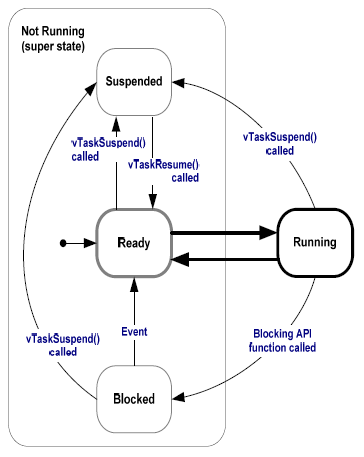
\includegraphics[width=0.3\textwidth]{Pictures/FreeRTOSOrg/taskStates.png}
	\caption{Task States. Quelle~\protect\citeA{MasteringFreeRtos}}
	\label{fig:TaskStates}
\end{figure}
Auf einem uProzessor mit einem Kern kann sich immer nur eine Task im Running Zustand befinden. Alle Tasks im Ready Zustand sind bereit und warten auf ihre Ausführung durch den Scheduler. Tasks die sich im Blocked Zustand befinden sind nicht bereit und warten auf ein Synchronisations- oder ein Timer Event. Eine Task die vTaskSuspend() aufruft, wird vom Scheduling Vorgang ausgeschlossen und nimmt den Zustand Suspended an. Erst nach den Aufruf von vTaskResume() verlässt die Task den Suspended Zustand.  Welche Task als nächstes vom Zustand Ready in den Zustand Running wechselt, wird durch den Schedulingalgorithmus bestimmt. Der Schedulingalgorithmus des FreeRTOS Kernels basiert auf Round Robin\cite{9783827373427}. Alle Tasks gleicher Priorität werden in einer Liste verwaltet. Jede Task in der Liste erhält ein gewisses Zeitquantum, welches bestimmt wie lange einer Task der Prozessor zugeteilt wird. Nach Ablauf des Zeitquantum wird ein Kontextwechsel durchgeführt und die nächste Task in der Liste erhält Prozessorzeit. Die Ausgelaufene Task wird durch den Scheduler automatisch hinten an die Liste angefügt. 
\begin{lstlisting}[caption={Pre-emptive List selection aus Task.c}, linewidth=8cm,captionpos=b, label=lst:nextTask, float=hbt]
#define taskSELECT_HIGHEST_PRIORITY_TASK(){																									
	UBaseType_t uxTopPriority = uxTopReadyPriority;														
		/* Find the highest priority queue that contains ready tasks. */								
		while(listLIST_IS_EMPTY(&(pxReadyTasksLists[ uxTopPriority ]))){																								
			configASSERT( uxTopPriority );																
			--uxTopPriority;																			
		}																								
		/* listGET_OWNER_OF_NEXT_ENTRY indexes through the list, so the tasks of						
		the	same priority get an equal share of the processor time. */									
		listGET_OWNER_OF_NEXT_ENTRY(pxCurrentTCB, &(pxReadyTasksLists[uxTopPriority]));			
		uxTopReadyPriority = uxTopPriority;																
	} /* taskSELECT_HIGHEST_PRIORITY_TASK */
\end{lstlisting}
Da in FreeRTOS jeder Task eine gewisse Priorität zugewiesen wird, gibt es auch für jede Priorität genau eine Liste. Der FreeRTOS Scheduling Algorithmus kann durch Konfigurations Präprozessor-defines angepasst werden. Der Scheduler kann entweder im Cooperative Modus oder im Preemption Modus ausgeführt werden. Die Konfiguration wird durch das define configUSE\_PREEMPTION geändert. Im Preemtive Modus wird eine aktive Task mit niedriger Priorität sofort von einer Task mit höherer Priorität verdrängt und ein Kontextwechsel wird durchgeführte. Im kooperativen Modus hingegen wird ein Taskwechsel erst durchgeführt, wenn eine Task den Prozessor explizit abgibt z.B. durch TaskYield(). Abbildung \ref{fig:PreVSCo} zeigt den Vergleich beider Modis durch einen beispielhaften Ablauf. Eine weitere Option die sich über das define configUSE\_TIME\_SLICING aktivieren lässt ist das sogenannte Zeitschlitzverfahren. Durch das Zeitschlitzverfahren wird die zugeteilte Prozessorzeit für Task gleicher Priorität gleichmäßig aufgeteilt. Dies geschieht durch Einführung fester TickInterrupt Intervalle. Bei jedem TickInterrupt überprüft der Scheduler ob sich eine Task gleicher Priorität im Ready Zustand befindet. Sollte es eine solche Task geben wird ein Kontextwechsel durchgeführt und die Task erhält den Prozessor zugeteilt. Die häufigst verwendete Scheduling Algorithmus nennt sich Prioritized Pre-emptive Scheduling with Time Slicing.
\begin{figure}[ht!]
	\centering
		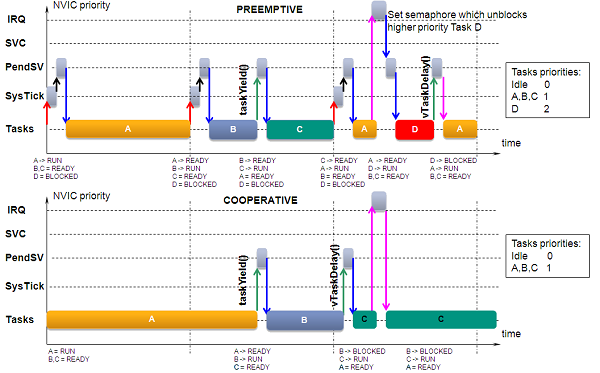
\includegraphics[width=0.5\textwidth]{Pictures/EMCUIT/PreemptiveCooperative.png}
	\caption{Pre-emptive vs. Co-operative. Quelle~\protect\citeA{MasteringFreeRtos} - Not referenced yet}
	\label{fig:PreVSCo}
\end{figure}

\begin{itemize}
	\item Tickcount
	\item FSM
	\item IDLE Task
	\item Priorität nicht durch Scheduler
\end{itemize}

\begin{lstlisting}[caption={Implementierung von SysTick aus Task.c}, linewidth=8cm,captionpos=b, label=lst:SysTickS, float=hbt]
void xPortSysTickHandler( void ){
	/* The SysTick runs at the lowest interrupt priority, so when this interrupt
	executes all interrupts must be unmasked.  There is therefore no need to
	save and then restore the interrupt mask value as its value is already
	known. */
	portDISABLE_INTERRUPTS();
	{
		/* Increment the RTOS tick. */
		if( xTaskIncrementTick() != pdFALSE )
		{
			/* A context switch is required.  Context switching is performed in
			the PendSV interrupt.  Pend the PendSV interrupt. */
			portNVIC_INT_CTRL_REG = portNVIC_PENDSVSET_BIT;
		}
	}
	portENABLE_INTERRUPTS();
}
\end{lstlisting}


\begin{lstlisting}[caption={Implementierung von Kontextwechsel aus Task.c}, linewidth=8cm,captionpos=b, label=lst:taskSwitch, float=hbt]
void vTaskSwitchContext( void )
{
	if( uxSchedulerSuspended != ( UBaseType_t ) pdFALSE )
	{
		/* The scheduler is currently suspended - do not allow a context
		switch. */
		xYieldPending = pdTRUE;
	}
	else
	{
		xYieldPending = pdFALSE;
		/* Check for stack overflow, if configured. */
		taskCHECK_FOR_STACK_OVERFLOW();
		/* Select a new task to run using either the generic C or port
		optimised asm code. */
		taskSELECT_HIGHEST_PRIORITY_TASK();
		traceTASK_SWITCHED_IN();
	}
}
\end{lstlisting}



\begin{figure}[ht!]
	\centering
		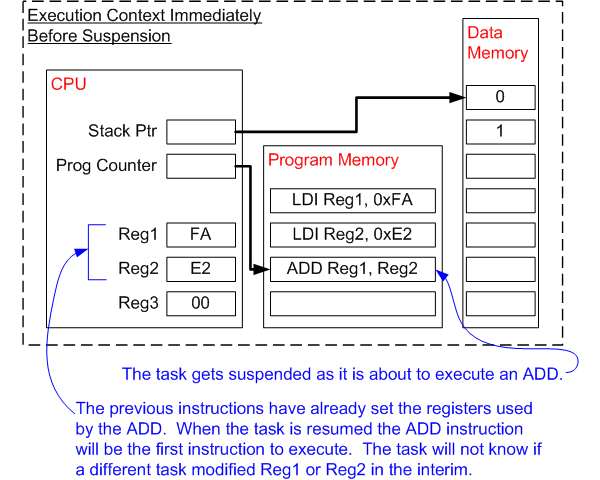
\includegraphics[width=0.4\textwidth]{Pictures/FreeRTOSOrg/ExeContext.png}
	\caption{FreeRTOS Pseudoimplementierung des Context - Switch. Quelle~\protect\citeA{MasteringFreeRtos} - Not referenced yet}
	\label{fig:FreeRTOSFsm}
	
\end{figure}

\begin{figure}[ht!]
	\centering
		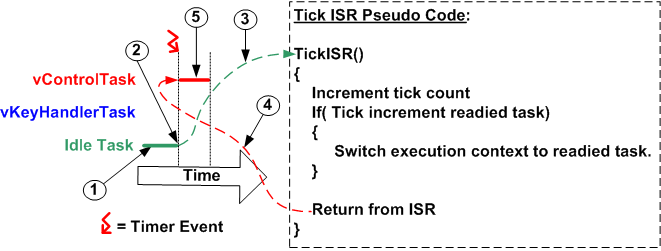
\includegraphics[width=0.4\textwidth]{Pictures/FreeRTOSOrg/TickISR.png}
	\caption{FreeRTOS Pseudoimplementierung des Tick Interrupts. Quelle~\protect\citeA{MasteringFreeRtos} - Not referenced yet}
	\label{fig:FreeRTOSFsm}
\end{figure}